\section{Methodology}\label{sec:methodology}

We aim to improve the performance of Neural Architecture Search (NAS) with reinforcement learning (RL) by using meta-learning. We, therefore, build a meta-RL system that can learn across environments and adapt to them. We split the system into two components: the NAS variables and the reinforcement learning framework. For the reinforcement learning framework, we make use of a deep meta-RL algorithm that follows the same line of \textit{Learning to reinforcement learn}~\citep{LtRL} and \textit{RL$^2$}~\citep{RL2}, with some minor adaptations in the meta-data employed and the design of the episodes. The environments that we consider are neural architecture design tasks for different datasets sampled from the meta-dataset collection~\citep{MetaDataset}. On the other hand, for the NAS elements, we work with a slightly modified version of the search space of BlockQNN~\citep{BlockQNN} and similarly, we use the test accuracy after early-stop training as the reward associated with the sampled architectures. In the remainder of the section, we discuss these elements further.%In the remainder of the section we discuss the elements of this approach further.


% For the reinforcement learning framework, we make use of a deep-meta reinforcement learning algorithm that follows the same line of \textit{Learning to reinforcement learn}~\citep{LtRL} and \textit{RL$^2$}~\citep{RL2}, with some minor adaptations in the meta-data that is used and the design of the episodes. The environments that we consider are neural architecture design tasks for different datasets sampled from the meta-dataset collection~\citep{MetaDataset}. On the other hand, for the NAS elements we work with a slightly modified version of the search space of BlockQNN~\citep{BlockQNN} and we use the test accuracy after early-stop training as the reward associated to the sampled architectures. In the remainder of the section, we discuss these elements further.

\subsection{The Neural Architecture Search elements}\label{sec:methodology:nas}

As described in Section~\ref{sec:preliminaries:nas}, three NAS variables characterize a research work in this area: the search strategy, the search space, and the performance estimation strategy. In our case, we constrain the search strategy to a deep meta-reinforcement learning algorithm that we explain in detail in Section~\ref{sec:methodology:rl}, and thus, here we only elaborate on the remaining two. 

\subsubsection{The search space}\label{sec:methodology:nas:ss}

The set of architectures considered in our work is inspired by BlockQNN~\citep{BlockQNN}, which defines the search space as all architectures that can be generated by sequentially stacking $d \in \mathbb{N}$ vectors from a so-called Network Structure Code (NSC) space containing encodings of the most relevant layers for CNNs. An NSC vector has information of the type of a layer, the value of its most important hyperparameter, its position on the network, and the allowed incoming connections (i.e., the inputs) so that it becomes possible to represent any architecture as a list of NSCs. The NSC definition is flexible in that it can easily be modified or extended and, moreover, it allows us to define an equivalent discrete action space for the reinforcement learning agent as described in Section~\ref{sec:methodology:rl:as}.

In Table~\ref{tab:methodology:nas:ss:nsc}, we present the NSC space for our implementation. Given a list of NSC vectors representing an architecture, the network is built following the next rules: firstly, based on BlockQNN's results, if a \textit{convolution} layer is found then a Pre-activation Convolutional Cell\footnote{The PCC stacks a ReLU, a convolution, and a batch normalization unit.} (PCC)~\citep{PCC} with 32 units\footnote{The selection of the number of units is made to reduce the cost of the training of the networks.} is used; secondly, the \textit{concatenation} and \textit{addition} operations create padded versions of their inputs if they have different shapes; thirdly, if at the end of the building process the network has two or more leaves then they get merged with a \textit{concatenation} operation\footnote{The last two rules do not apply for chain-structured architectures since no merge operations are needed.}. Figure~\ref{fig:methodology:nas:ss:rules} illustrates these rules.

\begin{figure}[ht]
\begin{center}
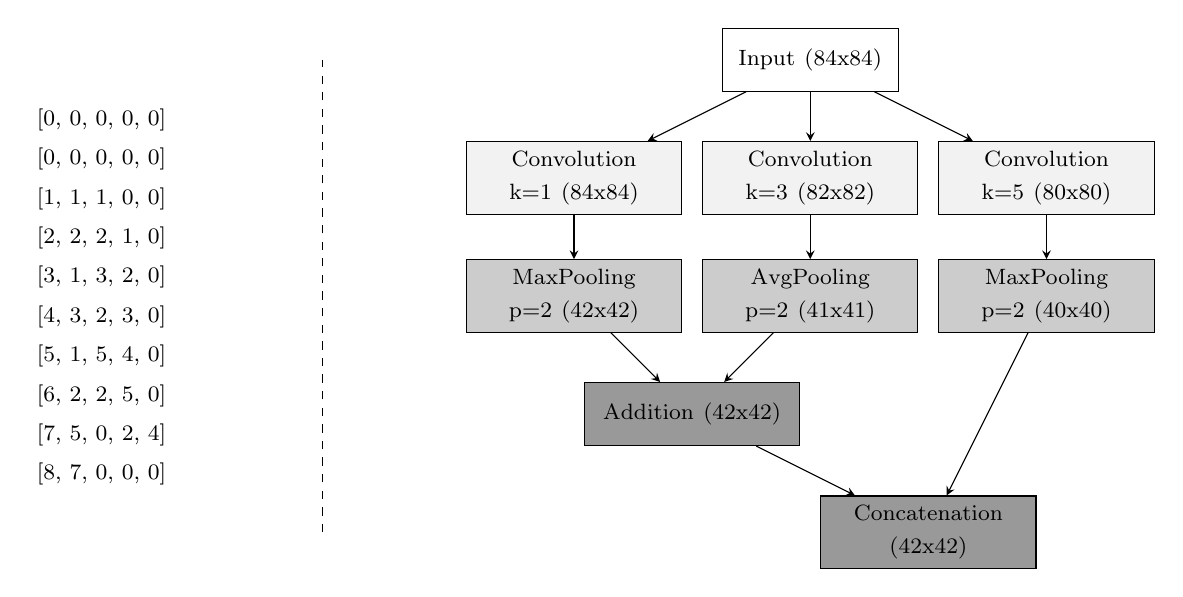
\begin{tikzpicture}
% NSC list
\node[align=left, below] at (0,-.5){\footnotesize [0, 0, 0, 0, 0]};
\node[align=left, below] at (0,-1.0){\footnotesize [0, 0, 0, 0, 0]};
\node[align=left, below] at (0,-1.5){\footnotesize [1, 1, 1, 0, 0]};
\node[align=left, below] at (0,-2.0){\footnotesize [2, 2, 2, 1, 0]};
\node[align=left, below] at (0,-2.5){\footnotesize [3, 1, 3, 2, 0]};
\node[align=left, below] at (0,-3.0){\footnotesize [4, 3, 2, 3, 0]};
\node[align=left, below] at (0,-3.5){\footnotesize [5, 1, 5, 4, 0]};
\node[align=left, below] at (0,-4.0){\footnotesize [6, 2, 2, 5, 0]};
\node[align=left, below] at (0,-4.5){\footnotesize [7, 5, 0, 2, 4]};
\node[align=left, below] at (0,-5.0){\footnotesize [8, 7, 0, 0, 0]};

% separator
\draw[dashed] (2.8, -6) -- (2.8, 0);

% definitions
\tikzstyle{input} = [rectangle, minimum width=2cm, minimum height=0.8cm, text centered, draw=black, fill=gray!0, text width=2cm]


\tikzstyle{convolution} = [rectangle, minimum width=2cm, minimum height=0.8cm, text centered, draw=black, fill=gray!10, text width=2.5cm]

\tikzstyle{maxpool} = [rectangle, minimum width=2cm, minimum height=0.8cm, text centered, draw=black, fill=gray!40, text width=2.5cm]

\tikzstyle{avgpool} = [rectangle, minimum width=2cm, minimum height=0.8cm, text centered, draw=black, fill=gray!40, text width=2.5cm]

\tikzstyle{concat} = [rectangle, minimum width=2cm, minimum height=0.8cm, text centered, draw=black, fill=gray!80, text width=2.5cm]

\tikzstyle{arrow} = [->,>=stealth]

% the graph
\node (l0) [input] at (9,0) {\footnotesize Input (84x84)};

\node (l1) [convolution, below of=l0, xshift=-3cm, yshift=-0.5cm] {\footnotesize Convolution k=1 (84x84)};

\node (l3) [convolution, below of=l0, yshift=-0.5cm] {\footnotesize Convolution k=3 (82x82)};

\node (l5) [convolution, below of=l0, xshift=3cm, yshift=-0.5cm] {\footnotesize Convolution k=5 (80x80)};

\node (l2) [maxpool, below of=l1, yshift=-0.5cm] {\footnotesize MaxPooling p=2 (42x42)};

\node (l4) [avgpool, below of=l3, yshift=-0.5cm] {\footnotesize AvgPooling p=2 (41x41)};

\node (l6) [maxpool, below of=l5, yshift=-0.5cm] {\footnotesize MaxPooling p=2 (40x40)};

\node (l7) [concat, below of=l2, yshift=-0.5cm, xshift=1.5cm] {\footnotesize Addition (42x42)};

\node (l8) [concat, below of=l7, yshift=-0.5cm, xshift=3.0cm] {\footnotesize Concatenation (42x42)};


\draw [arrow] (l0) -- (l1);
\draw [arrow] (l0) -- (l3);
\draw [arrow] (l0) -- (l5);

\draw [arrow] (l1) -- (l2);
\draw [arrow] (l3) -- (l4);
\draw [arrow] (l5) -- (l6);

\draw [arrow] (l2) -- (l7);
\draw [arrow] (l4) -- (l7);

\draw [arrow] (l7) -- (l8);
\draw [arrow] (l6) -- (l8);

\end{tikzpicture}
\caption{Example of an architecture sampled from the search space of our approach. On the left, a list of Neural Structure Codes (NSCs); on the right, the corresponding network after the application of the rules. For the sake of simplicity, in this example, the convolutions are assumed to have one filter only.}
\label{fig:methodology:nas:ss:rules}
\end{center}
\end{figure}

%TODO: cite the "most relevant" layers/types by maybe pointing to papers of the original networks considered.

%


%On the other hand, to avoid high-dimensional blocks that can cause memory issues for the multi-branch structures, we do not consider the \textit{concatenation} operation as a possible action for the reinforcement learning agent, but instead we use it as a merge operation when the delivered network has more than one leaf, as it is exemplified in Figure~\ref{fig:concat-merge}.


% Please add the following required packages to your document preamble:
% \usepackage{booktabs}
\begin{table}[ht]
\centering
\begin{tabular}{@{}cccccc@{}}
\toprule
\textbf{Name}   & \textbf{Index}  & \textbf{Type} & \textbf{Kernel size\footnotemark{}} & \textbf{Predecessor 1} & \textbf{Predecessor 2} \\ \midrule
Convolution     & \textbf{T}      & 1             & \{1, 3, 5\}          & \textbf{K}             & $\emptyset$            \\
Max Pooling     & \textbf{T}      & 2             & \{2, 3\}             & \textbf{K}             & $\emptyset$            \\
Average Pooling & \textbf{T}      & 3             & \{2, 3\}             & \textbf{K}             & $\emptyset$            \\
Addition        & \textbf{T}      & 5             & $\emptyset$          & \textbf{K}             & \textbf{K}             \\
Concatenation   & \textbf{T}      & 6             & $\emptyset$          & \textbf{K}             & \textbf{K}             \\
Terminal        & \textbf{T}      & 7             & $\emptyset$          & $\emptyset$            & $\emptyset$            \\ \bottomrule
\end{tabular}
\caption{The subset of the NSC space used, presented as in BlockQNN~\citep{BlockQNN}. The changes with respect to the original BlockQNN space are: a) the \textit{identity} operator (\textbf{Type} 4) is omitted; b) the pool size values changed from the original set $\{1, 3\}$ to $\{2, 3\}$ because a pool size of 1 does not contribute to any reduction. The set $\textbf{T}=\{1, 2 \dots , d \}$ refers to the position of each layer in the network, where $d$ is the maximum depth, and $\textbf{K} = \{0, 1, 2, \dots , \text{current layer index} - 1 \}$ the index of its predecessor. }
\label{tab:methodology:nas:ss:nsc}
\end{table}

\footnotetext{The kernel size is an attribute for the convolutions, whereas for the pooling elements it refers to the layer's pool size.}

\subsubsection{The performance estimation strategy}\label{sec:methodology:nas:pss}

Our estimation of the long-term performance of the designed networks closely follows the early-stop approach of BlockQNN-V1~\citep{BlockQNN}, but we ignore the penalization of the network's FLOPs and density since we have empirically ascertained that it is too strict when the classification task is difficult (i.e., when low accuracy values are expected).

The choice of an early-stop strategy is made to help reduce the computational cost of our approach. In short, for every sampled architecture $\mathcal{N}$ a prediction module is appended, and the network is then trained for a small number of epochs to obtain its accuracy on a test set, which is the final estimation of its long-term performance. The datasets considered are balanced, and their train and test splits are designed beforehand (see Section~\ref{sec:methodology:rl:environments}). % assumed to have been designed beforehand, and we  that the datasets' classes are balanced so that accuracy measures the performance well.

As in BlockQNN, for the prediction module we stack a fully-connected dense layer with 1024 units and ReLU activation function, a dropout layer with rate of 0.4, a dense layer with the number of units equals to the desired number of classes to predict and linear activation function, and a softmax that outputs the probabilities per class. The training is performed to minimize the cross-entropy loss using the Adam Optimizer~\citep{Adam} with the parameters used in BlockQNN: $\beta_1=0.9$, $\beta_2=0.999$, $\epsilon_{\textsc{adam}}=10e^{-8}$, and $\alpha_\textsc{adam}=0.001$ that is reduced by a factor of 0.2 every five epochs. After training, the network is evaluated on a test set by fixing the network's weights and selecting the class with the highest probability to be the final prediction per observation in the set so that the standard accuracy $\text{ACC}_{\mathcal{N}}$ can be returned.

\subsection{The reinforcement learning framework}\label{sec:methodology:rl}

The deep-meta-RL framework that we propose is different from standard RL in two main aspects. First, the \textit{agent} is challenged to face more than one \textit{environment} during training, and second, the distribution over the \textit{reward} domain learned by the agent is now dependant on the whole history of \textit{states}, \textit{actions}, and \textit{rewards}, instead of the simple \textit{state-action} pairs. 
%This distribution is approximated by an algorithm that models the \textit{policy} as a Recurrent Neural Network (RNN) that, thanks to its internal dynamics, is able to adapt to different environments to achieve its goal efficiently~\citep{LtRL}.
In the remainder of the section, we describe each of the RL elements.


\subsubsection{The states}\label{sec:methodology:rl:states}

A state $x_i \in \mathcal{X}$ is a multidimensional array of size $d \times 5$, storing $d$ NSC vectors sorted by layer index.
While this representation is programmatically easy to control, it is not ideal in a machine learning setting. In particular, we note that every element of an NSC vector is a categorical variable. Therefore, when required, every NSC vector in $x_t$ is transformed as follows: 
the layer's type\footnote{This size is the result of having 7 types of layers (see Section~\ref{sec:methodology:nas:ss}) plus the type 0 representing an empty layer.} is encoded into a one-hot vector of size 8, the predecessors into a one-hot vector of size $(d+1)$, and the kernel size into a one-hot vector of size $(k+1)$ with $k=\max(\text{kernel\_size})$. The transformation ignores the layer index because the state implicitly incorporates the information of the position of each layer due to sorting. This encoding results in a multidimensional array\footnote{When working with chain-structured networks the second predecessor is always omitted, reducing the dimensionality of the encoding to $d \times (d + k + 10)$.} of size $d \times (2d + k + 11)$. Figure~\ref{fig:methodology:rl:states:img} illustrates this transformation.

\begin{figure}[ht]
\begin{center}
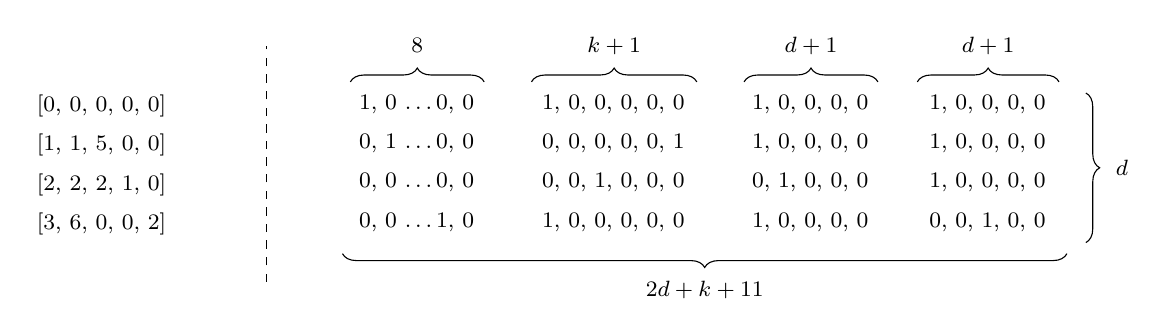
\begin{tikzpicture}

% The NSC list
\node[align=left, below] at (0,-.5){\footnotesize [0, 0, 0, 0, 0]};
\node[align=left, below] at (0,-1){\footnotesize [1, 1, 5, 0, 0]};
\node[align=left, below] at (0,-1.5){\footnotesize [2, 2, 2, 1, 0]};
\node[align=left, below] at (0,-2){\footnotesize [3, 6, 0, 0, 2]};

%%%%%%%% The encoding

\draw[dashed] (2.1, -3) -- (2.1, 0);

%l1
\node[align=left, below] at (4,-.5){\footnotesize 1, 0 \dots 0, 0};
\node[align=left, below] at (6.5,-.5){\footnotesize 1, 0, 0, 0, 0, 0};
\node[align=left, below] at (9,-.5){\footnotesize 1, 0, 0, 0, 0};
\node[align=left, below] at (11.25,-.5){\footnotesize 1, 0, 0, 0, 0};

%l2
\node[align=left, below] at (4,-1){\footnotesize 0, 1 \dots 0, 0};
\node[align=left, below] at (6.5,-1){\footnotesize 0, 0, 0, 0, 0, 1};
\node[align=left, below] at (9,-1){\footnotesize 1, 0, 0, 0, 0};
\node[align=left, below] at (11.25,-1){\footnotesize 1, 0, 0, 0, 0};

%l3
\node[align=left, below] at (4,-1.5){\footnotesize 0, 0 \dots 0, 0};
\node[align=left, below] at (6.5,-1.5){\footnotesize 0, 0, 1, 0, 0, 0};
\node[align=left, below] at (9,-1.5){\footnotesize 0, 1, 0, 0, 0};
\node[align=left, below] at (11.25,-1.5){\footnotesize 1, 0, 0, 0, 0};

%l4
\node[align=left, below] at (4,-2){\footnotesize 0, 0 \dots 1, 0};
\node[align=left, below] at (6.5,-2){\footnotesize 1, 0, 0, 0, 0, 0};
\node[align=left, below] at (9,-2){\footnotesize 1, 0, 0, 0, 0};
\node[align=left, below] at (11.25,-2){\footnotesize 0, 0, 1, 0, 0};

% The notes

\draw [decorate,decoration={brace,amplitude=5pt,raise=4pt},xshift=-4pt,yshift=0pt]
(12.5,-0.6) -- (12.5,-2.5) node [black,midway,xshift=0.6cm]{\footnotesize $d$};

\draw [decorate,decoration={brace,amplitude=5pt,mirror,raise=4pt},xshift=-4pt,yshift=0pt]
(3.2,-2.5) -- (12.4,-2.5) node [black,midway,yshift=-0.6cm]{\footnotesize $2d + k + 11$};

\draw [decorate,decoration={brace,amplitude=5pt,raise=4pt},xshift=-4pt,yshift=0pt]
(3.3,-0.6) -- (5.0,-0.6) node [black,midway,yshift=0.6cm]{\footnotesize $8$};

\draw [decorate,decoration={brace,amplitude=5pt,raise=4pt},xshift=-4pt,yshift=0pt]
(5.6,-0.6) -- (7.7,-0.6) node [black,midway,yshift=0.6cm]{\footnotesize $k+1$};

\draw [decorate,decoration={brace,amplitude=5pt,raise=4pt},xshift=-4pt,yshift=0pt]
(8.3,-0.6) -- (10,-0.6) node [black,midway,yshift=0.6cm]{\footnotesize $d+1$};

\draw [decorate,decoration={brace,amplitude=5pt,raise=4pt},xshift=-4pt,yshift=0pt]
(10.5,-0.6) -- (12.3,-0.6) node [black,midway,yshift=0.6cm]{\footnotesize $d+1$};

\end{tikzpicture}
\caption{The different representations of a state. In this example, a state $x_t$ contains $d=4$ NSC vectors. On the left, a network as a list of NSC vectors; on the right, the same network in its encoded representation. In our work, $k=5$ as observed in Table~\ref{tab:methodology:nas:ss:nsc}.}
\label{fig:methodology:rl:states:img}
\end{center}
\end{figure}

% TODO: make a figure maybe

\subsubsection{The action space}\label{sec:methodology:rl:as}

We formulate the action space $\mathcal{A}$ as a discrete space of 14 actions listed in Table~\ref{tab:methodology:rl:as}. Each action $a_i \in \mathcal{A}$ can either append a new element from the NSC space to a state $x_j \in \mathcal{X}$ or control two pointers, $p_1$ and $p_2$, for the indices of the predecessors to use for the next NSC vector. We note that for the chained-structured networks no pointers are required since the predecessor is always the previous layer, and neither do the merging operations \textit{addition} and \textit{concatenation}, making it possible to reduce the action space to 8 actions only.

% \usepackage{booktabs}
\begin{table}[ht]
\centering
\begin{tabular}{@{}cl@{}}
\toprule
\textbf{Action ID} & \textbf{Description}                                                               \\ \midrule
A0                  & Add \textit{convolution} with $\text{kernel\_size}=1$, using predecessor $p_1$     \\
A1                  & Add \textit{convolution} with $\text{kernel\_size}=3$, using predecessor $p_1$     \\
A2                  & Add \textit{convolution} with $\text{kernel\_size}=5$, using predecessor $p_1$     \\
A3                  & Add \textit{max-pooling} with $\text{pool\_size}=2$, using predecessor $p_1$       \\
A4                  & Add \textit{max-pooling} with $\text{pool\_size}=3$, using predecessor $p_1$       \\
A5                  & Add \textit{avg-pooling} with $\text{pool\_size}=2$, using predecessor $p_1$       \\
A6                  & Add \textit{avg-pooling} with $\text{pool\_size}=3$, using predecessor $p_1$       \\
A7                  & Add \textit{terminal} state.                                                       \\
A8                  & Add \textit{addition} with predecessors $p_1$ and $p_2$                            \\
A9                  & Add \textit{concatenation} with predecessors $p_1$ and $p_2$                       \\
A10                 & Shift $p_1$ one position up (i.e., $p_1 = p_1 + 1$)                                                        \\
A11                 & Shift $p_1$ one position down (i.e., $p_1 = p_1 - 1$)                                                  \\
A12                 & Shift $p_2$ one position up (i.e., $p_2 = p_2 + 1$)                                                        \\
A13                 & Shift $p_2$ one position down (i.e., $p_2 = p_2 - 1$)                                                      \\ \bottomrule
\end{tabular}
\caption{The action space proposed, which is compliant with the NSC space of section~\ref{sec:methodology:nas:ss}. %For the chain-structured networks the space contains only actions 0-7 since the predecessor is always known to be the previous layer.
}
\label{tab:methodology:rl:as}
\end{table}


\subsubsection{The environments}\label{sec:methodology:rl:environments}

In our work, an environment is a neural architecture design task for image classification on a specific dataset of interest. The goal for an agent on this environment is to come up with the best architecture possible after interacting for a certain number of time-steps. At any time-step $t$, the environment's state is $x_t \in \mathcal{X}$, which is the NSC representation of a neural network $N_t$. The reward $r_t \in [0, 1]$ associated with $x_t$ is a function of the network's accuracy $\text{ACC}_{N_t} \in [0, 1]$ (Section~\ref{sec:methodology:nas:pss}). The initial state $x_0$ of the environment is an empty architecture. 

An agent can interact with the environment through a set of episodes by performing actions $a_t \in \mathcal{A}$. In our terminology, an \textit{episode} is the trajectory from a reset of the environment's state until a termination signal. The environment triggers the termination signal in the following cases: a) the predecessors $p_1$ and $p_2$ are out of bounds after the execution of $a_t$, b) $a_t$ is a \textit{terminal} action, c) $x_t$ contains $d$ NSC elements (the maximum depth) after performing $a_t$, d) the total number of actions executed in the current episode is higher than a given number $\tau$, or e) the action led to an invalid architecture. The agent-environment interaction process is formalized in Algorithm~\ref{alg:methodology:rl:environments:interaction}.

\begin{algorithm}
% \label{alg:methodology:rl:environments:interaction}
\caption{Agent-environment interaction}\label{euclid}
\begin{algorithmic}[1]
    \Procedure{interact}{Agent, Environment, Dataset, $t_{max}$, $\sigma$}
    \State $done \gets \text{False}$
    \State $t \gets 0$
    \State $\text{Environment.reset\_to\_initial\_state()}$
    \While {$t < t_{max}$}
        \State $a_t \gets \text{Agent.get\_next\_action()}$
        \State $x_t \gets \text{Environment.update\_state(}a_t\text{)}$
        \State $N \gets \text{Environment.build\_network(}x_t\text{)}$
        \State $\text{ACC}_{N_t} \gets \text{N.accuracy(Dataset)}$
        \If{$a_t$ is shifting}
            \State $r_t \gets \sigma \cdot \text{ACC}_{N_t}$ 
            % \State $t \gets t + 1$
        \Else
            \State $r_t \gets \text{ACC}_{N_t}$ 
        \EndIf
        
        \State $done \gets \text{Environment.is\_termination()}$ \label{alg:methodology:rl:environments:interaction:termination}
        
        \State $\text{Agent.learn(}x_t, a_t, r_t, done\text{)}$
        
        \If{$done$}
            \State $ \text{Environment.reset\_to\_initial\_state()}$
            \State $done \gets \text{False}$
        \EndIf
    \EndWhile
    \EndProcedure
    
\end{algorithmic}
\label{alg:methodology:rl:environments:interaction}
\end{algorithm}

As mentioned in the beginning of Section~\ref{sec:methodology}, we work with more than one environment. Specifically, we define five environments, each one associated with a different dataset sampled from the meta-dataset collection~\citep{MetaDataset}. The datasets are listed in Table~\ref{tab:methodology:environments:datasets} and they were selected as explained in Appendix~\ref{app:datasets}. All datasets have balanced classes. In order to evaluate the accuracy of a network $N_t$, for any dataset we perform a deterministic 1/3 train-test split and follow the pre-processing that has been initially proposed by the meta-dataset authors so that the images are resized to a shape of $84 \times 84 \times 3$ using bilinear interpolation. 

\begin{table}[ht]
\centering
\begin{tabular}{@{}ccccc@{}}
\toprule
Dataset ID    & Dataset name                              & Usage      & N classes & N observations \\ \midrule
aircraft      & FGVC-Aircraft                             & Validation & 100       & 10000          \\
cu\_birds     & CUB-200-2011                              & Validation & 200       & 11788          \\
dtd           & Describable Textures                      & Train      & 47        & 5640           \\
omniglot      & Omniglot                                  & Train      & 1623      & 32460          \\
vgg\_flower   & VGG Flower                                & Train      & 102       & 8189           \\ \bottomrule
\end{tabular}
\caption{List of datasets considered for the environments. They are sampled from the meta-dataset~\citep{MetaDataset} as explained in Appendix \ref{app:datasets}.}.
\label{tab:methodology:environments:datasets}
\end{table}

\subsubsection{Deep meta-reinforcement learning}\label{sec:methodology:rl:dmrl}

Our deep meta-RL approach, illustrated in Figure~\ref{fig:methodology:rl:formal:diag}, is based on the work of~\citet{LtRL} and~\citet{RL2}. They propose to learn a policy that, in addition to the \textit{state-action} pairs of standard RL, uses the current time-step in the agent-environment interaction (the temporal information) as well as the previous action and reward. In this way, the agent can learn the relation between its past decisions and the current action. However, we introduce a modification in the temporal information, by considering the relative step within an episode instead of the global time-step so that the agent can capture the relation between changes in a neural architecture.

Formally, let $\mathcal{D}$ be a set of Markov Decision Processes (MDPs). Consider an agent embedding a Recurrent Neural Network (RNN) - with internal state $h$ - modeling a policy $\pi$. At the start of a \textit{trial}, a new task $m_i \in \mathcal{D}$ is sampled, and the internal state $h$ is set to zeros (empty network). The agent then executes its action-selection strategy for a certain number $t_{max}$ of discrete time-steps, performing $n$ episodes of maximum length $l$ depending on the environment's rules. At each step $t$ (with $0 \leq t \leq t_{max}$) an action $a_t \in A$ is executed as a function of the observed history $H_t = \{x_0, a_0, r_0, c_0, . . . , x_{t-1}, a_{t-1}, r_{t-1}, c_{t-1}, x_t\}$ (set of states $\{x_s\}_{0 \leq s \leq t}$, actions $\{a_s\}_{0 \leq s < t}$, rewards $\{r_s\}_{0 \leq s < t}$, episode-related steps $\{c_s\}_{0 \leq s \leq l}$) and a reward $r_t$ is obtained. At the very beginning of the trial, the action $a_0$ is sampled at random from a uniform distribution of all actions available, and the state $x_0$ is given by the environment's rules. The RNN's weights are trained to maximize the total discounted reward accumulated during each \textit{trial}. The evaluation consists of resetting $h$ and fixing $\pi$ to run an interaction with a new MDP $m_e \not\in \mathcal{D}$.

\begin{figure}[ht]
\begin{center}
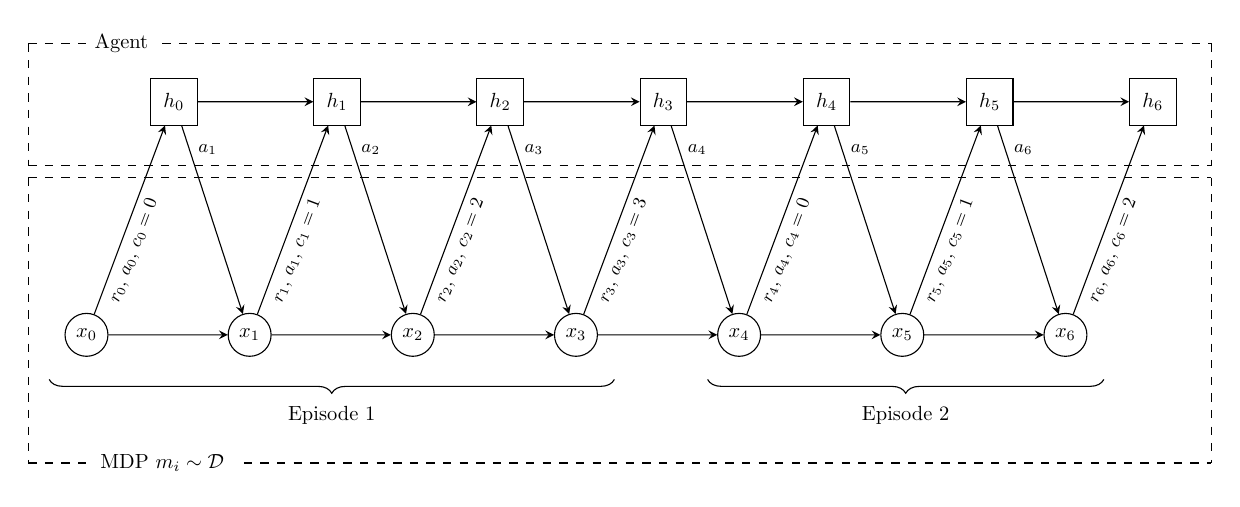
\begin{tikzpicture}[scale=0.74, every node/.style={scale=0.74}]

% definitions
\tikzstyle{hidden} = [rectangle, minimum width=0.8cm, minimum height=0.8cm, text centered, draw=black]


\tikzstyle{state} = [circle, radius=0.8, text centered, draw=black]

\tikzstyle{arrow} = [->,>=stealth]

% box top
\draw[dashed] (-2.5, 0) -- (-2.5, -2.1); % left
\draw[dashed] (-2.5, 0) -- (-1.5, 0); % topA
\node at (-0.9, 0){Agent}; % Label
\draw[dashed] (-0.2, 0) -- (17.8, 0); % topB
\draw[dashed] (-2.5, -2.1) -- (17.8, -2.1); % bottom
\draw[dashed] (17.8, 0) -- (17.8, -2.1); % right


% box bottom
\draw[dashed] (-2.5, -2.3) -- (-2.5, -7.2); %left
\draw[dashed] (-2.5, -2.3) -- (17.8, -2.3); % top
\draw[dashed] (-2.5, -7.2) -- (-1.5, -7.2); % bottomA
\node at (-0.2, -7.2){ MDP $m_i \sim \mathcal{D} $}; % Label
\draw[dashed] (1.2, -7.2) -- (17.8, -7.2); % bottomB
\draw[dashed] (17.8, -2.3) -- (17.8, -7.2); % right

% hidden states
\node (h0) [hidden] at (0, -1){ $h_0$};

\node (h1) [hidden, right of=h0, xshift=1.8cm]{ $h_1$};

\node (h2) [hidden, right of=h1, xshift=1.8cm]{ $h_2$};

\node (h3) [hidden, right of=h2, xshift=1.8cm]{ $h_3$};

\node (h4) [hidden, right of=h3, xshift=1.8cm]{ $h_4$};

\node (h5) [hidden, right of=h4, xshift=1.8cm]{ $h_5$};

\node (h6) [hidden, right of=h5, xshift=1.8cm]{ $h_6$};

\node (x1) [state, below of=h0, xshift=1.3cm, yshift=-3cm]{ $x_1$};

\node (x0) [state, left of=x1, xshift=-1.8cm]{ $x_0$};

\node (x2) [state, right of=x1, xshift=1.8cm]{ $x_2$};

\node (x3) [state, right of=x2, xshift=1.8cm]{ $x_3$};

\node (x4) [state, right of=x3, xshift=1.8cm]{$x_4$};

\node (x5) [state, right of=x4, xshift=1.8cm]{ $x_5$};

\node (x6) [state, right of=x5, xshift=1.8cm]{$x_6$};

\draw [arrow] (h0) -- (h1);
\draw [arrow] (h1) -- (h2);
\draw [arrow] (h2) -- (h3);
\draw [arrow] (h3) -- (h4);
\draw [arrow] (h4) -- (h5);
\draw [arrow] (h5) -- (h6);

\draw [arrow] (x0) -- (h0) node[near start,below, sloped, xshift=0.4cm] {\small $r_0$, $a_0$, $c_0=0$};

\draw [arrow] (x1) -- (h1) node[near start,below, sloped, xshift=0.4cm] {\small $r_1$, $a_1$, $c_1=1$};

\draw [arrow] (x2) -- (h2) node[near start,below, sloped, xshift=0.4cm] {\small $r_2$, $a_2$, $c_2=2$};

\draw [arrow] (x3) -- (h3) node[near start,below, sloped, xshift=0.4cm] {\small $r_3$, $a_3$, $c_3=3$};

\draw [arrow] (x4) -- (h4) node[near start,below, sloped, xshift=0.4cm] {\small $r_4$, $a_4$, $c_4=0$};

\draw [arrow] (x5) -- (h5) node[near start,below, sloped, xshift=0.4cm] {\small $r_5$, $a_5$, $c_5=1$};

\draw [arrow] (x6) -- (h6) node[near start,below, sloped, xshift=0.4cm] {\small $r_6$, $a_6$, $c_6=2$};

\draw [arrow] (h0) -- (x1) node[near start, right, yshift=0.4cm, xshift=-0.1cm] {\small $a_1$};

\draw [arrow] (h1) -- (x2) node[near start,right, yshift=0.4cm, xshift=-0.1cm] {\small $a_2$};

\draw [arrow] (h2) -- (x3) node[near start,right, yshift=0.4cm, xshift=-0.1cm] {\small $a_3$};

\draw [arrow] (h3) -- (x4) node[near start,right, yshift=0.4cm, xshift=-0.1cm] {\small $a_4$};

\draw [arrow] (h4) -- (x5) node[near start,right, yshift=0.4cm, xshift=-0.1cm] {\small $a_5$};

\draw [arrow] (h5) -- (x6) node[near start,right, yshift=0.4cm, xshift=-0.1cm] {\small $a_6$};

% arrows between states
\draw [arrow] (x0) -- (x1);
\draw [arrow] (x1) -- (x2);
\draw [arrow] (x2) -- (x3);
\draw [arrow] (x3) -- (x4);
\draw [arrow] (x4) -- (x5);
\draw [arrow] (x5) -- (x6);

\draw [decorate,decoration={brace,amplitude=5pt,mirror,raise=4pt},xshift=-4pt,yshift=-5pt]
(-2,-5.4) -- (7.7,-5.4) node [black,midway,yshift=-0.8cm]{Episode 1};

\draw [decorate,decoration={brace,amplitude=5pt,mirror,raise=4pt},xshift=-4pt,yshift=-5pt]
(9.3,-5.4) -- (16.1,-5.4) node [black,midway,yshift=-0.8cm]{Episode 2};


\end{tikzpicture}
\caption{A graphic representation, inspired by the RL$^2$ illustration~\citep{RL2}, of our deep meta-reinforcement learning framework. In this example, the trial consists of $t_{max}=6$ time-steps, and the agent is able to complete two episodes of different length. $c_s$ is a counter of the current step in the episode and it gets reset at the start of any new episode. The states $x_0$ and $x_4$ are shown to be different, although in practice the initial state of an episode could always be the same.}
\label{fig:methodology:rl:formal:diag}
\end{center}
\end{figure}


\subsubsection{The policy optimization algorithm}\label{sec:methodology:rl:poa}

Similarly to~\citet{LtRL}, we make use of the synchronous Advantage Actor-Critic (A2C)~\citep{A2C} with one worker. As it can be observed in Figure~\ref{fig:related:rl:alg:lstm}, the only change in the A2C network is in the input of the recurrent unit, so that the updates of the network's parameters remain unchanged.

\begin{figure}[ht]
\begin{center}
\begin{tikzpicture}

\tikzstyle{point} = []
\tikzstyle{box} = [rectangle, text centered, draw=black]

\tikzstyle{arrow} = [->,>=stealth]

\node (x) [point] at (0, 0){\footnotesize$x_t$};


\node (enc) [box, below of=x, text width=1.2cm]{\footnotesize State encoder};

\node (flat) [box, below of=enc]{\footnotesize Flatten};

\node (oenc) [box, right of=enc, text width=1.2cm, xshift=0.8cm]{\footnotesize One-hot encoder};

\node (a) [point, above of=oenc]{\footnotesize$a_{t-1}$};

\node (r) [point, right of=a, xshift=0.2cm]{\footnotesize$r_{t-1}$};
\node (c) [point, right of=r]{\footnotesize$c_{t}$};

\node (con) [box, below of=flat, xshift=1.8cm, minimum width=5cm]{\footnotesize Concatenation};

\node (lstm) [box, below of=con, minimum width=1.5cm]{ $\circlearrowright$};

\node (pi) [point, below of=lstm, xshift=-1cm]{\footnotesize $\pi(a_t | s_t; \theta)$};

\node (v) [point, below of=lstm, xshift=1cm]{\footnotesize $V(s_t; \theta_v)$};

\draw [arrow] (x) -- (enc);

\draw [arrow] ($(flat)+(0, -0.25)$) -- ($(con)+(-1.8, 0.25)$);
\draw [arrow] (a) -- (oenc);
\draw [arrow] (oenc) -- ($(con)+(0, 0.25)$);

\draw [arrow] (r) -- ($(con)+(1.2, 0.25)$);
\draw [arrow] (c) -- ($(con)+(2.2, 0.25)$);
\draw [arrow] (enc) -- (flat);

\draw [arrow] (con) -- (lstm);

\draw [arrow] (lstm) -- (pi);
\draw [arrow] (lstm) -- (v);


\end{tikzpicture}
\caption{Illustration of the \textit{meta}-A2C architecture. In our implementation, the ``State encoder" follows the procedure explained in  Section~\ref{sec:methodology:rl:states}, and the recurrent layer is an LSTM with 128 units.}
\label{fig:related:rl:alg:lstm}
\end{center}
\end{figure}

Formally, let $t$ be the current time step, $s_t=x_t \cdot a_{t-1} \cdot r_{t-1} \cdot c_t$ a concatenation of inputs, $\pi(a_t|s_t; \theta)$ the policy, $V(s_t; \theta_v)$ the value function, $H$ the entropy, $j \in \mathbb{N}$ the horizon, $\gamma \in (0, 1]$ the discount factor, $\eta$ the regularization coefficient, and $R_t = \sum_{i=0}^{j-1} \gamma^i r_{t+i}$ the total accumulated return from time step $t$. The gradient of the objective function is:
\begin{equation}
    \nabla_{\theta} \log \pi(a_t|s_t;\theta) \underbrace{(R_t - V(s_t; \theta_v))}_\textrm{Advantage estimate} + \underbrace{\eta \nabla_{\theta}H(\pi(s_t; \theta))}_\textrm{Entropy regularization}
\end{equation}\label{eq:methodology:rl:poa:gradient}

As it is usually the case for A2C, the parameters $\theta$ and $\theta_v$ are shared except for the ones in output layers. For a detailed description of the algorithm, we refer to the original paper~\citep{A2C}.
